%arara : pdflatex
\documentclass[12pt]{article}

\usepackage{../../TP0/style}

\begin{document}
\def\reportnumber{3}
\def\reporttitle{Algorithmes de Complexité temporelle quadratique O(n²)}
%----------------------------------------------------------------------------------------
%	TITLE PAGE
%----------------------------------------------------------------------------------------


\begin{titlepage} % Suppresses displaying the page number on the title page and the subsequent page counts as page 1
	\newcommand{\HRule}{\rule{\linewidth}{0.5mm}} % Defines a new command for horizontal lines, change thickness here
	
	\center % Centre everything on the page
	
	%------------------------------------------------
	%	Headings
	%------------------------------------------------
	
	\baselineskip=2\baselineskip 
	\textsc{\LARGE Université des Sciences et de la Technologie Houari Boumediene}%\\[1cm] % Main heading such as the name of your university/college

	%------------------------------------------------
	%	Logo
	%------------------------------------------------
	
	%\vfill\vfill
	\vfill
	
\includegraphics[width=0.3\textwidth]{../style/USTHB_Logo.png}\\[1cm] % Include a department/university logo - this will require the graphicx package
	 
	%----------------------------------------------------------------------------------------
	
	\textsc{\Large Compilation}\\[0.5cm] % Major heading such as course name
	%\textsc{\large Minor Heading}\\[0.5cm] % Minor heading such as course title
	
	%------------------------------------------------
	%	Title
	%------------------------------------------------
	
	\HRule\\[0.4cm]
	\baselineskip=1.2\baselineskip 
	{\huge\bfseries Rapport de Projet \\
	 \reporttitle}\\[0.4cm] % Title of your document
	
	\HRule\\[1.5cm]
	
	%------------------------------------------------
	%	Author(s)
	%------------------------------------------------
	
	\begin{minipage}{0.4\textwidth}
		\begin{flushleft}
			\large
			\textit{Binôme: groupe 4}\\
			HOUACINE  \textsc{Naila Aziza} % Your name
			\\
			MOHAMMEDI \textsc{Haroune } % Your name
			
		\end{flushleft}
	\end{minipage}
	~
	\begin{minipage}{0.4\textwidth}
		\begin{flushright}
			\large
			\textit{Professeur}\\
			Mme. MEKAHLIA \textsc{Fatma Zohra} % Supervisor's name
		\end{flushright}
	\end{minipage}
	
	%------------------------------------------------
	%	Date
	%------------------------------------------------
	
	\vfill\vfill\vfill % Position the date 3/4 down the remaining page
	
	{\large\today} % Date, change the \today to a set date if you want to be precise
	
	
	\vfill % Push the date up 1/4 of the remaining page
	
\end{titlepage}


\section{Partie I: Algorithme 1 du test de la primalité.}

\subsection{Développement de l'algorithme de Tri par sélection d'un tableau de (n$>$=2) éléments. }

\begin{sql}

 FONCTION Tri_Selection(T:Tableau[] , n:entier):Tableau[]
VAR
	i,j,n1,x : entier;
DEBUT
	i = 1;
	n1 = n -1;
	
	TANT QUE(i <= n1)
	FAIRE
		j = i +1;
		
		TANT QUE(j <= n)
		FAIRE
			
			SI( T[i] > T[j] )
			ALORS
				x = T[i] ;
				T[i] = T[j];
				T[j] = x;
			FIN SI;
			
			j = j + 1;
			
		FAIT;
		i = i + 1;	
	FAIT;
	retourner T;

FIN
 
\end{sql}

\subsection{Complexité:}

\subsubsection{Calcule des complexités temporelles en notation asymptotique de Landau O (Grand O) de  cet  algorithme au meilleur cas, notée f1(n), et au pire cas, notée f2(n). }

 
\begin{enumerate}
	\item Calcule de la complexité au meilleur cas:
	\\
	Il s'agit du cas ou le tableau est déjà trié dans l'ordre croissant, tel que :
	\\
	f1(n) = 1(=) + 2(-,=) + n($<$=) + (n-1)*2(+,=) + $\frac{n^2+n-2}{2}$ + $\frac{n^2+n-2}{2}-1 + 2*\frac{n^2+n-2}{2}$ + (n-1)*2(+,=) + 1(return).
	\\ 
	\color{blue}
	f1(n) = 2$n^2$ + 7n - 5 (Opérations) $\Rightarrow$ f1(n) = O($n^2$)
	\color{black}
	\\
	\item Calcule de la complexité au pire cas:
	\\
	Il s'agit du cas ou le tableau est trié dans l'ordre inverse (ordre décroissant), tel que :\\
	f2(n) = 1(=) + 2(-,=) + n($<$=) + (n-1)*2(+,=) + $\frac{n^2+n-2}{2} + \frac{n^2+n-2}{2}-1 + 3*(\frac{n^2+n-2}{2}-1) + 2*\frac{n^2+n-2}{2}$ + (n-1)*2(+,=) + 1(return).
	\\

	\color{blue}
	f2(n) = $\frac{7n^2}{2}$ + $\frac{17n}{2}$ + - 11 (Opérations) $\Rightarrow$ f2(n) = O($n^2$)
	\color{black}
\end{enumerate}
\texttt{ }\\

\color{red}
REMARQUE:\\

\color{black}
Nous remarquons que dans le pire est le meilleur des cas la complexité temporelle est toujours de l'ordre de O($n^2$).


\subsubsection{Calculer la complexité spatiale en notation exacte et en notation asymptotique de Landau O (Grand O) de  cet  algorithme notée s(n).}
Il s'agit du nombre de case mémoire ou octets utilisés par le programme.
\\
Pour calculer la complexité spatiale de cet algorithme nous allons considérer les tailles mémoires des types en langage C; tel que nous aurons:
int/entier : 2 octets
\\
\begin{enumerate}
	\item En notation exacte:
	\\
Nous avons dans cet algorithme cinq (5) variables de type "entier" en plus d'un tableau de n entiers.
\\
Ce qui nous fait :
\color{blue}
 (n + 5)(2 octets) = 2n + 10 octets
\color{black}
\\
 
	\item En notation asymptotique:
	\\
	Le nombre de case mémoire dépend uniquement de la taille du tableau, donc on obtient:
	\\
	\color{blue}
	s(n) = O(n)
	\color{black}
	
	
\end{enumerate}



\subsection{Développement de programme correspondant avec le langage C.}
\subsubsection{Procédure de Tri}
\begin{sql}
void selectionSort(long int *t, long int n){
    long int i,j,min,imin;
    for(i=0;i<n-1;i++){
        imin=i;
        for(j=i+1;j<n;j++){
           if(t[imin]>t[j]){
              min=t[j];
              imin= j;
           }
        }
        if(imin != i){
           t[imin]=t[i];
           t[i]=min;
        }
    }
}
\end{sql}

\subsubsection{Quelques fonctions d'aide pour les trois (3) type de tableaux. }

Fonction de création et de calcule du temps d'exécution de la fonction de tri pour un tableau comportant des données en ordre Croissant.
\begin{sql}
double sortedTime(long int n) {
    
  long int *array = malloc(n*sizeof(long int));
  long int i;
  
  for (i = 0; i < n; i++)
  {
      array[i] = i;
  }
  clock_t start = clock();
  selectionSort(array, n); //replace with your function 
  clock_t end = clock();
  
  return (double) (end - start)/CLOCKS_PER_SEC;
}

\end{sql}

Fonction de création et de calcule du temps d'exécution de la fonction de tri pour un tableau comportant des données en ordre inverse (décroissant). 
\begin{sql}
double inversedTime(long int n) {
    
  long int *array = malloc(n*sizeof(long int));
  long int i;
  
  for (i = 0; i < n; ++i)
  {
    array[i] = n - i;
  }
  clock_t start = clock();
  selectionSort(array, n); //replace with your function 
  clock_t end = clock();

  return (double) (end - start)/CLOCKS_PER_SEC;
}
\end{sql}

Fonction de création et de calcule du temps d'exécution de la fonction de tri pour un tableau comportant des données en ordre Aléatoire
\begin{sql}
double randomTime(long int n) {
    
  long int *array = malloc(n*sizeof(long int));
  long int i;
  
  for (i = 0; i < n; ++i)
  {
    array[i] = (int) rand()%n;
  }
  clock_t start = clock();
  selectionSort(array, n); //replace with your function 
  clock_t end = clock();

  return (double) (end - start)/CLOCKS_PER_SEC;
}
\end{sql}

Fonction de récupération des résultats des temps d'exécution dans un fichier.
\begin{sql}
  void saveResults(double array[], long int n, char* name) {

     long int i;
     FILE * fp;
     fp = fopen ("tp3_results","a");
     fprintf(fp, name);
     fprintf(fp, "[");

     for(i = 0;i<n;i++) {
      fprintf(fp, "%lf, ",array[i]);
     }

     fprintf(fp, "]\n");
     fclose (fp);
  }
\end{sql}

\subsubsection{Algorithme de teste }
Lancement de l'algorithme pour les différentes tailles de tableau et avec les 3 type de tableaux (ordonné , ordre inverse , aléatoire).

\begin{sql}
#include <stdio.h>
#include <stdbool.h>
#include <stdlib.h>
#include<time.h>

int nbInputs = 12;
long int inputs[] = {50000 , 100000 , 200000 , 400000 , 800000 , 3200000 , 6400000 , 12800000 , 25600000 , 1024000000 , 2048000000};
         
int main(int argc, char const *argv[])
  {
  double *inversedTimes = malloc(nbInputs*sizeof(double));
  double *sortedTimes = malloc(nbInputs*sizeof(double));
  double *randomTimes = malloc(nbInputs*sizeof(double));
  int i;

  for (i = 0; i < nbInputs; i++)
  {
    inversedTimes[i] = inversedTime(inputs[i]);
    sortedTimes[i] = sortedTime(inputs[i]);
    randomTimes[i] = randomTime(inputs[i]);
  }

  saveResults(inversedTimes,nbInputs, "inversed = ");
  saveResults(sortedTimes,nbInputs, "sorted = ");
  saveResults(randomTimes,nbInputs, "random = ");

  return 0;
  }
\end{sql}

\subsubsection{Résultat}
Ansin dans le fichier \texttt{tp3\_results} on obtiendra les résultats suivants:
\begin{sql}
inversed = [5.308000, 21.059000, 87.593000, 342.122000, 1368.488000,
 5446.582000, 22330.988000, 93790.146170,373284.781800, 1530467.605000,
  6106565.745000  ]
  
sorted = [4.813000, 19.649000, 79.942000, 318.696000, 1274.784000, 
5736.528000, 22946.112000, 94996.908000, 436985.756900 , 1747943.028000,
 7201525.274000 ]
 
random = [5.025000, 20.328000, 81.150000, 292.308000, 1169.232000, 
4817.235840, 19172.59864, 76690.394570, 322099.657200, 1285177.632000,
 5654781.582000 ]
\end{sql}

\subsection{Mesure des temps d'exécution.}
Grâce à l'exécution du programme C vu précédemment nous avons obtenu les temps d'exécution des trois (3) cas de tableaux.

\subsubsection{Remplissage du tableau:}
\color{blue}
\textrm{  }
\\
\\
\begin{tabular}{|p{3cm}||p{1.8cm}|p{1.8cm}|p{1.8cm}|p{1.8cm}|p{1.8cm}|p{1.8cm}|}
\hline
Taille du Tableau (N) : & 50000 & 100000 & 200000 & 400000 & 800000  & 1600000\\
\hline
Temps (bon ordre) : & 3.190 & 12.533 & 49.868 & 218.696 & 846.771 & 4736.528 \\
\hline

Temps (ordre inverse) :  & 3.263 & 13.000 & 52.035 & 242.122 & 918.292 & 4446.582 \\
\hline

Temps (Aléatoire) : & 3.133 & 12.563 & 50.082 & 192.308 & 857.088 & 3817.235 \\
\hline
\end{tabular}
\\
\\
\begin{tabular}{|p{3cm}||p{2cm}|p{2cm}|p{2cm}|p{2cm}|p{2cm}|}
\hline
Taille du Tableau (N) : & 3200000 & 6400000 & 12800000 & 25600000 &  51200000  \\
\hline

Temps (bon ordre) : & 22946.112 & 94996.908 & 436985.756 & 1747943.028 & 7201525.274  \\
\hline

Temps (ordre inverse) : &  22330.988 & 93790.146 & 373284.781 & 1530467.605 &  6106565.745  \\
\hline

Temps (Aléatoire) : & 19172.598 & 76690.394 & 322099.657 & 1285177.632 & 5654781.582  \\
\hline
\end{tabular}


\textrm{  }
\\
\color{black}





\subsection{Représentation par un graphe, Gf1(n) et Gf2(n), les variations de la fonction de la complexité temporelle correspondant au meilleur cas f1(n) et au pire cas f2(n) en fonction de n respectivement; et par trois (3) autres graphes,  les variations  du temps d'exécution T(n) en fonction de n selon les trois (3) type d'ordre du tableau.}
\texttt{  }\\

\subsubsection{Représentation des graphes de la variation du temps d'exécution :}


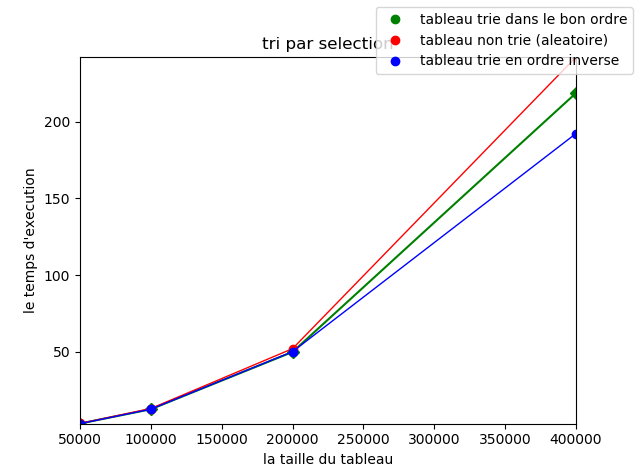
\includegraphics[width=1\textwidth]{graphe/Tri_selection.png}

\subsubsection{Représentation des deux graphes Gf1 et Gf2 du meilleur et pire cas respectivement :}

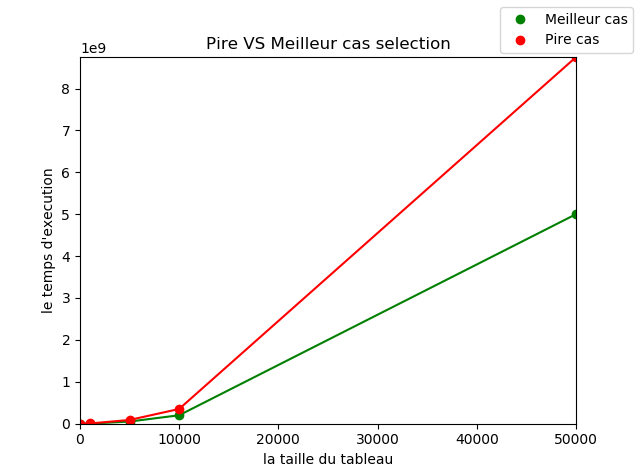
\includegraphics[width=1\textwidth]{graphe/Pire_Meilleur_Selection.png}


\subsection{Interprétation des résultats.}
\subsubsection{Comparaison des mesures de temps d'exécution avec le pire et meilleur cas:}
	  
Vu que la complexité au pire et meilleur cas sont identiques, il est claire que les temps d'exécutions suivent la même évolution, en O($n^2$).

\subsubsection{Remarque et déduction d'une fonction T(n) reliant n au temps d'exécution.}

On remarque que les temps d'exécution sont approximativement multipliés par 4 lorsque N est doublé n'importe l'ordre des éléments du tableau.
\\

\color{blue}
Exemples:
\color{black} 
\\
N1 = $50000  \Rightarrow  $  T1 = 3.190
\\
N2 = $100000 \approx 2 * N1  \Rightarrow  $  T2 = 13.533 $\approx 4 * T1 $
\\

Aussi
\\
N1 = $400000 \Rightarrow $  T1 = 218.696
\\
N2 = $800000 \approx 2 * N1 \Rightarrow $  T2 = 849.771 $\approx 4 * T1 $
\\

On en déduit que le temps d'exécution est proportionnel à N, ce que l'on peut représenter par la formule suivante
: 
\begin{center}
\color{red}
	$T(x*N) = x^2*T(N)$ pour tous $ x*N \in [50000 - 2048000000] $	
	
\color{black}
(x étant la tangente d'un point sur le graphe).
\end{center}

Nous ne pouvant pas généraliser car les testes que nous avons fait n'englobent pas toutes les valeurs possibles, 
	



\subsubsection{Comparaison de la complexité théorique et expérimentale. }
Dans le cas des données de l'échantillon la complexité théorique et expérimentale sont du même ordre de grandeur que la complexité théorique du pire et meilleur cas,\\
\color{blue}
Donc Le modèle théorique est conforme aux mesures expérimentales.
\color{black}
\\
\texttt{  }
\\
Même si en générale la complexité expérimentale d'un échantillon quelconque est compris entre la complexité au pire cas et au meilleur cas.
\\
\texttt{  }
\\
\begin{center}
\color{blue}
Complexité Meilleur cas = complexité expérimentale = complexité Pire cas 
\color{black}
\end{center}

\end{document}
